\section{Stretching Constraint Controller}
\label{sec:stretching_constraint_controller}

\todoin{Update notation throughout - including figures}
\todoin{Make algorithm block}

% \begin{algorithm}[ht]
%     \caption{LocalConstrainedController$(\robotconfig, \deformconfig, \deformtarget, \relaxeddistancematrix, \stretchmax)$}
%     \begin{algorithmic}[1]
%         \State $\correspondences \gets$ CalculateCorrespondences$(\deformconfig_t, \deformtarget)$
%         \State $\deformvel_e, \Pinvweight_e \gets$ FollowNavigationFunction$(\deformconfig_n, \correspondences)$
%         \State $\robotcommandvel \gets$ FindBestConstrainedRobotMotion$(\robotconfig, \deformconfig, \deformvel_e, \Pinvweight_e)$
%     \end{algorithmic}
%     \label{alg:local_constrained_controller}
% \end{algorithm}

While the controller in the previous section has had some success at preventing excessive stretching~\cite{Berenson2013}, it is not able to prevent stretching when the grippers move on opposite sides of an obstacle (see attached video). To address this, we introduce a novel geometric constraint which is able to directly address the cause of overstretch.

\subsection{Overstretch}
\label{Method_Overstretch}
The stretching avoidance of the deformable object is formulate due to the compliant nature and the lack of control of the deformable object. In the previous section, a stretching correction term $\deformvel_s \in \deformVspace$ is applied when the object becomes overstretched. However, this method cannot handle cases where the object is caught on an obstacle.

We detect the overstretching (i.e. excessive strain) of the object by examining the value of the stretching ratio $\stretchcurr$, which denotes the maximum value among the ratio between the Euclidean distance $\| \straightvecIJ \|$ and the geodesic distance $\geodistIJ$ for every pair of points $\deformconfigI$ and $\deformconfigJ$:
\begin{equation}
    \stretchcurr = \max_{\substack{\deformidx, j \in 1, \dots, \ndeformpoints \\ j > \deformidx}} \frac{\| \straightvecIJ \|}{\geodistIJ}
    \label{Eq:Method_stretching_detection}
\end{equation}
we denote $\stretchmax$ as the maximum allowed stretching ratio. Our method initiates stretching-avoidance when $\stretchcurr > \stretchmax$.
\todoin{we've already defined $\stretchmax$ earlier.}

We assume that the object starts in an unstretched state, so the overstretch that arises is due to the motion of the grippers. Thus if we can constrain gripper motions to a set which does not overstretch the object further than a threshold, we can prevent or reduce the overstretch at the next time step. We know that the force causing the overstretch comes from the grippers, so if we reduce the length of geodesic paths through the object between grippers, the strain on the object should decrease. When overstretch is detected, we thus introduce a conical constraint for each gripper that shrinks the allowable $\grippervelG$ to reduce the length of the geodesics between the grippers. 

\begin{figure}[ht]
    \centering
    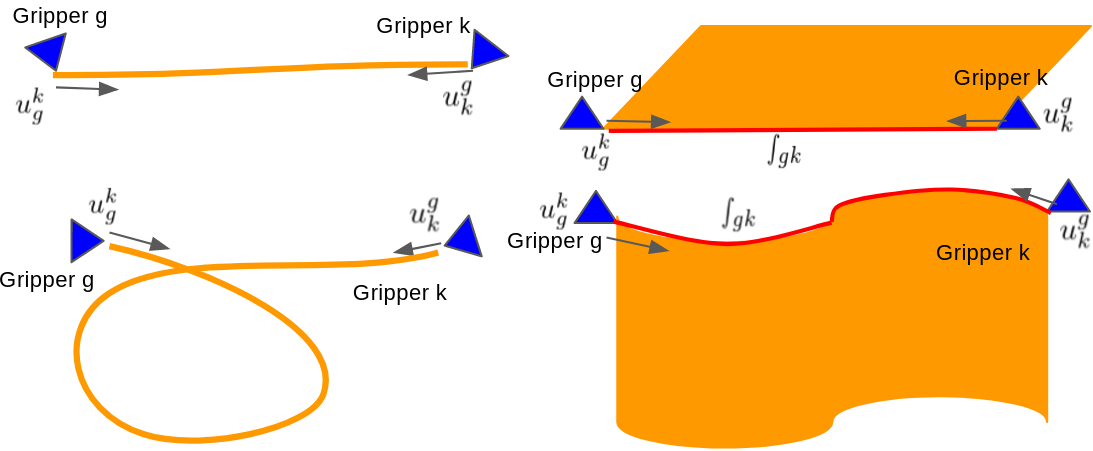
\includegraphics[width=.98\linewidth]{Stretching_vector_method.png}
    \caption{The arrows in gray show the direction of each stretching vector at the corresponding gripper with respect to the gripper pair $\gripperconfigG$ and $\gripperconfigK$. Left: stretching vectors on the rope when the rope is at rest (above) or is deformed (below). Right: stretching vectors on the cloth when the cloth is at rest (above) or is deformed (below). The red lines denote the geodesic connecting the corresponding $\deformconfigGK$ and $\deformconfigKG$ on the object.}
    \label{Fig:stretching_avoidance_vector_method}
\end{figure}

A conical constraint is constructed for each gripper and points along the \textit{stretching avoidance vector}, which is an estimation of the direction to move to decrease the strain. For a pair of grippers with index $\gripperidx$ and $k$, two stretching avoidance vectors are defined, one for each gripper. Let $\closestpointGK$ be the index of the point grasped by the $\gripperidx$th gripper, which has the minimum geodesic distance to the set of points grasped by $\gripperconfigK$. We define $\closestpointKG$ similarly.  Let $\geodesicGK$ be the geodesic on the object from $\deformconfigGK$ to $\deformconfigKG$. We denote $\savoidGK$ and $\savoidKG$ as the pair of stretching avoidance vectors on grippers $\gripperidx$ and $k$ respectively.  Then $u^k_g$ is the tangent vector of $\geodesicGK$ at $\deformconfigGK$ and $\savoidGK$ is the tangent vector of $\geodesicKG$ at the point $\deformconfigKG$ (as shown in Fig. \ref{Fig:stretching_avoidance_vector_method}). 

\todoin{Go through and revise notation for $C_s$ and $s$ etc.}

To specify the stretching constraint, we first define the function $s(\grippervelG, \gripperconfigG, \gripperconfigK, \deformconfig)$, which specifies the constraint on gripper $\gripperidx$ defined by the interaction of grippers $\gripperidx$ and $k$. Correspondingly, $\savoidGK$ is the stretching avoidance vector for gripper $\gripperidx$, which is the tangent vector of $\geodesicGK$ at $\deformconfigGK$. The larger the value of $s$, the more we expect geodesic path length between grippers will be reduced. Thus, $s$ should increase as $\angle (\grippervelG, \savoidGK)$ increases. Assume we wish to have a lower bound $s_s$ on $s$, then $C_s$ is a set of constraints $C_s = \{C_s^1, \dots, C_s^G\}$, where each constraint is:
\begin{equation}
    C_s^g =\{ \grippervelG\in \tanse3 \mid \forall k\neq g, \ s(\grippervelG, \gripperconfigG, \gripperconfigK, \deformconfig) \geq s_s  \}
    \label{Eq:Stretching_avoidance_Method}
\end{equation}
Many functions can satisfy the requirements of $s$. In our work, we specify the function as:
\begin{equation}
    s(\grippervelG, \gripperconfigG, \gripperconfigK, \deformconfig) = \cos \angle (\grippervelG, \savoidGK ) = \cos \angle (\transvelG, \savoidGK )
    \label{Eq:Stretching_avoidance_Method_This_Paper}
\end{equation}

\subsection{Collision} Collision avoidance for the robot is addressed by the constraint $C_c$, which is the set of motions that keeps the grippers away from obstacles:

\todoin{Replace this with reference to Proximity etc earlier}

\begin{equation}
    C_c = \left\{\grippervelG\in \tanse3 \mid  \dbuffer - l(\gripperconfigG) - \frac{\mathfrak{n}(\gripperconfigG) \cdot \grippervelG}{||\grippervelG||} \grippervelG \Delta t < 0\right\}
    \label{Eq:Collision_constraint_Method}
\end{equation}
where $l(\gripperconfigG)$ is the function returning the distance from the gripper to its closest obstacle. $\mathfrak{n}(\gripperconfigG)$ returns the unit surface normal of the obstacle closest to the $\gripperidx$th gripper. The idea is to make each gripper keep at least the safe distance away from the closest obstacle. While we consider free-flying grippers in this section, similar constraints can be imposed on the entire geometry of a robot arm to avoid collisions all along the arm as was done in Sec.~\ref{sec:figureoutwhattorefhere}.


\subsection{Optimization Method}

Given these constraints, we then formulate an optimization problem similar to Eq.~\eqref{eqn:jacobianbackwardfunction_sim}, replacing the approximate Jacobian model with the directional rigidity model (Sec.~\ref{sec:constrained_model}), and adding the new stretching and collision constraints.

\todoin{Replace $C_s$ and $C_c$ with something else more directly accurate}
\todoin{Confirm these max vel equations in the implementation}

\begin{equation}
\begin{aligned}
    \DeformBackwardFn(\deformvel, \Pinvweight) = 
        & \argmin{\grippervel}
            & & \| \DeformForwardFnFull - \deformvel_e \|_{\Pinvweight_e} \\
        & \textrm{subject to}
            & & \grippervel \in C_s\\
        &   & & \grippervel \in C_c\\
        &   & & \grippervelGnorm \leq \grippervelmaxservo \enspace, \quad \gripperidx = 1, \dots, \ngrippers
\end{aligned}
\label{Eq:Optimization Problem}
\end{equation}

Because our objective function is not necessarily convex, we used a custom optimization method to solve the problem specified in Eq. \ref{Eq:Optimization Problem}. Our method is a type of numerical gradient descent with an additional projection step to enforce constraints.

Our method's outer loop computes the numerical gradient of the objective function. An inner loop then performs backtracking line search to find the gradient step size. However, the gradient step may cross a constraint boundary, thus after we compute the step size, we check if any constraint has been violated after taking the step. If it has, we project the step back to the feasible space. A simple projection to the boundary of a violated constraint may satisfy that constraint but violate others. Instead, to perform the projection, we solve a convex optimization problem (using the Gurobi optimizer \cite{Gurobi2016}) to find the nearest feasible point. This is possible because all the constraints in our problem are convex. Once such a point is found, the outer loop continues to iterate until convergence.